\documentclass[a4paper, oneside]{discothesis}

\usepackage[utf8]{inputenc}
\usepackage[T1]{fontenc}
\usepackage{graphicx}
\usepackage{epstopdf}
\usepackage{epigraph}
\usepackage{amsmath}

\thesistype{Master's Thesis}
\title{Rethinking Adversarial Examples}

\author{Yahya Jabary}
\email{yjabary@ethz.ch}

\institute{Computer Engineering and Networks Laboratory \\[2pt] ETH Zürich}

% \logo{
\includegraphics[width=0.2\columnwidth]{figures/dsg-logo}}

\supervisors{Prof.\ Dr.\ Roger Wattenhofer\\[2pt] Prof.\ Dr.\ Schahram Dustdar}

\keywords{Robustness, Alignment, Interpretability, Algorithmic Models}
% \categories{ACM categories go here.}

\date{\today}

%
% extended config
%

\usepackage{mathtools}

\setlength\parindent{0pt}

% example boxes
% https://www.overleaf.com/latex/examples/simple-stylish-box-design/stzmmcshxdng
\usepackage[many]{tcolorbox}
\usepackage{mathspec}
\usepackage{setspace}
\usepackage{multicol}
\tcbset{sharp corners, colback = white, before skip = 0.5cm, after skip = 0.5cm, breakable}
\newtcolorbox{highlightbox}{sharpish corners, boxrule = 0pt, leftrule = 4.5pt, enhanced, breakable, fuzzy shadow = {0pt}{-2pt}{-0.5pt}{0.5pt}{black!35}}

%
% content
%

\begin{document}

\frontmatter % do not remove this line
\maketitle

\cleardoublepage

\begin{acknowledgements}
	This thesis comes from working on a problem that truly matters to me, in an environment where curiosity and passion were shared, and I felt a sense of belonging. The topic of adversarial examples reflects my journey well, highlighting how subtle differences in perspective can lead to vastly different interpretations and outcomes.

	I'm deeply grateful to those who supported me along the way. My parents, Shima and Florian, and my family, for their unwavering support, even when I took risks and turned down financial opportunities to pursue my passion. My partner, Laura, whose love and encouragement crossed the Atlantic and got me through many long nights.
	
	I owe much to those who made this work possible. Prof.\ Roger Wattenhofer, for trusting me with this project and guiding me with wisdom and humor. Andreas Plesner, who was just as much of a mentor as a collaborator, for his dedication to our vision. Turlan Kuzhagaliyev and Alireza Furutanpey, for their camaraderie.
	
	Thanks also to those whose paths have diverged from mine but whose impact remains with me: Prof.\ Schahram Dustdar, who enabled my studies abroad, and Prof.\ Ali Mashtizadeh, who introduced me to operating systems research.
	
	I hope to continue this journey with the same spirit that brought me here.
\end{acknowledgements}

\begin{abstract}
    % The abstract should be short, stating what you did and what the most important result is.
	...
\end{abstract}

\tableofcontents

\mainmatter % do not remove

\chapter{Introduction}

% good style: https://arxiv.org/pdf/2202.02435

We have two goals in writing this document. One: fulfilling the requirements for a master's degree by presenting and extending our original research~\cite{jabary2024seeing} in thesis form. Two: offering a fresh and cohesive perspective on the rapidly evolving and, in our view, really exciting field of adversarial machine learning to a broader audience, with fewer technical prerequisites. We hope it will be valuable to those interested.

\section{Definition}

Adversarial examples are closely related to the concept of perturbation methods\footnote{Thanks to Prof.\ Wattenhofer for sharing this piece of unorthodox history.}.

The origin of perturbations can be traced back to the early days of computational geometry by Seidel et al. in 1998~\cite{seidel1998nature}. Perturbation techniques in computational geometry address a fundamental challenge: handling ``degeneracies'' in geometric algorithms. These are special cases that occur when geometric primitives align in ways that break the general position assumptions the algorithms rely on.

\begin{highlightbox}
	\textbf{Example:} Perturbation scheme for a Linear Classifier \\

	Consider a simple case of determining whether a point lies above or below a line~\cite{de2000computational}. While this classification appears straightforward, numerical issues arise when the point lies exactly on the line. Such degeneracies can cascade into algorithm failures or inconsistent results. The elegant solution is to imagine slightly moving (perturbing) the geometric objects to eliminate these special cases. Formally, we can express symbolic perturbation as $p_\varepsilon(x) = x + \varepsilon \cdot \delta(x)$ where $x$ is the original input, $\varepsilon$ is an infinitesimally small positive number the exact value of which is unimportant, and $\delta(x)$ is the perturbation function to break degeneracies. \\

	A perturbation scheme should be (1) consistent, meaning that the same input always produces the same perturbed output (2) infinitesimal, such that perturbations are small enough not to affect non-degenerate cases and (3) effective, in breaking all possible degeneracies. \\

	One powerful perturbation approach is Simulation of Simplicity (SoS)~\cite{franklin2022implementing, edelsbrunner2002topological, edelsbrunner2001sink, edelsbrunner1990simulation, levy2016robustness, schorn1993axiomatic}. SoS systematically perturbs input coordinates using powers of a symbolic infinitesimal. For a point $p_i = (x_i, y_i)$, the perturbed coordinates become:

	$$(\tilde{x_i}, \tilde{y_i}) = (x_i + \varepsilon^{2i}, y_i + \varepsilon^{2i+1}) = p_i + \varepsilon^{2i} \cdot (1, \varepsilon)$$

	This scheme ensures that no two perturbed points share any coordinate, effectively eliminating collinearity and other degeneracies.
\end{highlightbox}

The beauty of perturbation methods lies in their ability to handle degeneracies without explicitly detecting them, making geometric algorithms both simpler and more robust.

Adversarial examples on the other hand, first introduced by Szegedy et al.\ in 2014~\cite{szegedy2013intriguing}, follow the same principles as perturbation methods, but with the opposite objective. Instead of seeking to eliminate degeneracies (brittleness in the decision boundary), they exploit them to cause targeted misclassifications. Intuitively they can be understood as seeking the closest point in the input space that lies on the ``wrong side'' of a decision boundary relative to the original input. This shift, applied to the original input, creates an adversarial example.

\begin{highlightbox}
	\textbf{Example:} Fast Gradient Sign Method (FGSM) \\

	FGSM is one of the earliest and most widely recognized adversarial attack techniques, introduced by Goodfellow et al.~\cite{goodfellow2014explaining} in the context of visual recognition tasks. Given an input image $x$, FGSM generates an adversarial example $x'$ by perturbing the input in the direction of the gradient of the loss function with respect to the input.\\

	The perturbation is controlled by a parameter $\varepsilon > 0$~\footnote{Commonly $\varepsilon = 8/255$ for 8-bit images, so it stays within the precision constraints of the pixel values.}, which determines the magnitude of the change based on the direction of change for each pixel or feature in the input $x$. The model's loss function denoted by $J$, $\theta$ represents the model's parameters, and $y$ is the true target label. \\
	
	It works by calculating the gradient of the loss function with respect to the input, $\nabla_x J(\theta, x, y)$, and then adjusting the input in the direction of this gradient. The sign of the gradient, $\text{sign}(\nabla_x J(\theta, x, y))$, is used to ensure that the perturbation is small, while the $\ell_\infty$-norm constraint ensures that the change to the input remains ``imperceptible'' to human observers~\cite{goodfellow2014explaining, zhang2019adversarial}. More on the concept of imperceptibility later.\\
	
	The process for generating an adversarial example with FGSM can be expressed as:
	
	$$x' = x + \underbracket{\varepsilon \cdot \text{sign}(\nabla_x J(\theta, x, y))}_{\text{Perturbation}}$$
	
	In the untargeted version, the perturbation is designed to increase the loss for the correct class. In the targeted version the perturbation is designed to minimize the loss with respect to the adversary's chosen target class, making the model predict it deliberately.
\end{highlightbox}

While initially discovered in computer vision applications, the attack can be crafted for any domain or data type, even graphs~\cite{Kashyap2024AdversarialAA}. Natural language processing models can be attacked by circumventing the discrete nature of text data~\cite{Han2022TextAA, meng2020geometry, yang2024assessing}. One particularly entertaining example is the subversion of the conference paper-reviewer assignment model by Eisenhofer et al.~\cite{eisenhofer2023no}, where authors preselect reviewers to gain a competitive advantage. Speech recognition systems are vulnerable to audio-based attacks, where crafted noise can cause system failure~\cite{rajaratnam2018noise}. Deep reinforcement learning applications, including pathfinding and robot control, have also shown susceptibility to adversarial manipulations that can compromise their decision-making capabilities~\cite{Bai2018AdversarialEC}.

\section{Threat Modeling}

Having established the general concept of adversarial examples, we can now explore the various ways they can be categorized. Our system is not exhaustive: The field continues to evolve, with new attack vectors emerging regularly~\cite{Khaleel2024AdversarialAI}. This is particularly important in threat modeling, where the goal is to anticipate and defend against potential attacks.

We can differentiate between white-box and black-box attacks. White-box attacks assume complete knowledge of and access to the target model, while black-box attacks operate with limited or no access to the model's internal workings~\cite{capozzi2024adversarial}. Interestingly, research has shown that in some cases, black-box attacks can be more effective than white-box approaches at compromising model security~\cite{capozzi2024adversarial}.

An attack can be targeted or untargeted. Targeted attacks aim to manipulate the model into producing a specific, predetermined output, whereas untargeted attacks simply seek to cause any misclassification or erroneous output~\cite{capozzi2024adversarial, Kashyap2024AdversarialAA}. This distinction is particularly relevant in security-critical applications, where the attacker's goals may vary from causing general disruption to achieving specific malicious outcomes.

The method used to generate adversarial examples can be gradient-based, optimization-based or search-based strategies. For example, some text-based attacks leverage language models to generate alternatives for masked tokens, ensuring grammatical correctness and semantic coherence~\cite{garg2020bae}.

The extent to which adversarial examples are transferable \textendash{} meaning their ability to fool multiple different models \textendash{} is another way to differentiate them. Some adversarial examples demonstrate high transferability across various model architectures, while others are more model-specific in their effectiveness~\cite{Li2022ASO, li2022review}. Recent research has shown that adversarial examples are more readily transferable between vanilla neural networks than between defended ones~\cite{li2019nattack, zheng2023black}.

Finally, the attacks can be either focused on preserving the semantic meaning of inputs or exploit the mathematical properties of models without regard for semantic interpretation provides~\cite{browne2020semantics}.

\section{Imperceptible $\not=$ Semantics Preserving}

Adversarial examples are traditionally expected to have two key properties: (1) they should successfully cause misclassification in machine learning models while (2) remaining imperceptible to human observers~\cite{cubuk2017intriguing}.

However, the concept of ``imperceptibility [to humans]'' as originally proposed by Szegedy et al.~\cite{szegedy2013intriguing} by limiting pixel-space perturbations through an $\varepsilon$-bounded constraint is fundamentally flawed. This is because the human visual system is not solely reliant on pixel-space information to interpret images~\cite{ ning2023hflic}:

\begin{figure}
    \centering
    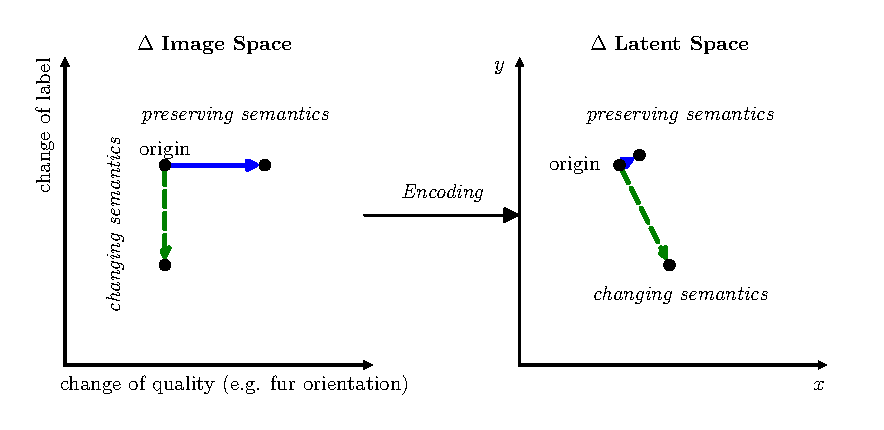
\includegraphics[width=1\columnwidth]{figures/latentspace.pdf}
    \caption{Semantics preserving/changing perturbations in pixel/latent-space.}
    \label{fig:latentspace}
\end{figure}

\begin{enumerate}
	\item \textit{Changing many pixels doesn't necessarily change semantics}: For instance, changes in lighting, exposure, sharpness, field of view or even the the orientation of an animal's fur~\cite{kilcher2021dimpled} does not necessarily alter the semantic content of an image, despite involving many pixel-space changes. The figure~\ref{fig:latentspace} serves to illustrate this point, assuming that the latent representations are perfectly aligned with the human judgement function.

	\item \textit{Changing few pixels doesn't necessarily preserve semantics}: The assumption that minimal pixel-space changes ensure semantic preservation is also flawed. This is because small $\varepsilon$-bounded adversarial perturbations are found to cause misclassification in time-constrained humans~\cite{elsayed2018adversarial}. Even more interestingly, humans detect forged low-$\varepsilon$ adversarial examples with high accuracy in both the visual (85.4\%)~\cite{veerabadran2023subtle} and textual ($\geq$70\%)~\cite{herel2023preserving} domain. Invertible neural networks can partially mitigate this issue in the visual domain~\cite{chen2023imperceptible}.
\end{enumerate}

\begin{highlightbox}
	\textbf{Open Question:} If imperceptibility is not a reliable indicator of semantic preservation, then what are the true properties of adversarial examples?
\end{highlightbox}

Recent research has shifted towards more nuanced concepts like ``semantic preservation''~\cite{careil2023towards} acknowledging that the relationship between perturbation size and semantic change is not straightforward. This shift has led to the development of new methods for generating adversarial examples that focus on preserving semantic information rather than relying on pixel-space constraints~\cite{lee2020semantics}.

The challenge of defining semantics remains central to this discussion. Without perfect representations that align with human judgment functions, we must rely on the best available encoders as proxies for semantic preservation~\cite{herel2023preserving}. This pragmatic approach acknowledges the limitations of current technology while striving for more meaningful adversarial examples.

\section{Inner Representations}

The internal latent representations of neural networks, their alignment with human understanding and the resuling gap between the two (the human-machine vision gap~\cite{geirhos2021partial}) is a central theme in adversarial machine learning research. This gap has many practical implications for the robustness and interpretability of machine learning models.

Neural networks trained with topological features develop substantially different internal representations compared to those trained on raw data, though these differences can sometimes be reconciled through simple affine transformations~\cite{mcguire2023neural}. This finding suggests that while the structural representations may differ, the underlying semantic understanding might be preserved across different training approaches.

The Centered Kernel Alignment (CKA) metric enables us to compare neural network representations, though it comes with important caveats. In biological and artificial neural networks, CKA can show artificially high similarity scores in low-data, high-dimensionality scenarios, even with random matrices~\cite{murphy2024correcting}. This limitation is particularly relevant when comparing representations of different sizes or when analyzing specific regions of interest.

The relationship between network architecture and concept representation has also been explored. Generally higher-level concepts are typically better represented in the final layers of neural networks, while lower-level concepts are often better captured in middle layers~\cite{Agafonov2022AnEO, Agafonov2022LocalizationOO}. This hierarchical organization mirrors our understanding of human cognitive processing and suggests that neural networks naturally develop structured representations that align with human conceptual understanding.

The choice of objective function significantly influences how networks represent information, particularly when dealing with biased data. Networks trained with Negative Log Likelihood and Softmax Cross-Entropy loss functions demonstrate comparable capabilities in developing robust representations~\cite{bangaru2022interpreting}.

Recent research~\cite{bansal2021revisiting} has demonstrated that neural networks with strong performance tend to learn similar internal representations, regardless of their training methodology. Networks trained through different approaches, such as supervised or self-supervised learning, can be effectively ``stitched'' together without significant performance degradation. This suggests a convergence in how successful neural networks represent information.

\begin{highlightbox}
	\textbf{Hypothesis:} ``Neural networks, trained with different objectives on different data and modalities, are converging to a shared statistical model of reality in their representation spaces.''~\cite{huh2024platonic}
\end{highlightbox}

This aligns with the ``Platonic Representation Hypothesis''~\cite{huh2024platonic}, which suggests that neural networks are converging toward a shared statistical model of reality, regardless of their training objectives or architectures. As models become larger and are trained on more diverse tasks and data, their internal representations increasingly align with each other, even across different modalities like vision and language. This convergence appears to be driven by the fundamental constraints of modeling the underlying structure of the real world, similar to Plato's concept of an ideal reality that exists beyond our sensory perceptions. The hypothesis proposes that this convergence is not coincidental but rather a natural consequence of different models attempting to capture the same underlying statistical patterns and relationships that exist in reality~\cite{huh2024platonic}. 

Should the ``Platonic Representation Hypothesis'' hold true, this would either mean that (a) adversarial examples as we know them are misalignments from a converged model of reality, or (b) that there exist a universal adversarial example that can fool any model, regardless of its architecture, training data or objective function, converging to a single and shared model of reality. Recent work by Moosavi-Dezfooli et al. \cite{moosavi2017universal} have demonstrated the existence of a single perturbation that can fool most models for all naturally occurring images, adding weight to the latter interpretation, though the question remains open.

\section{Counterintuitive Properties \& Mental Models}

The question discussed in the previous section is just one of many that remain open. In fact, there are several counterintuitive properties of adversarial examples that have yet to be fully explained:

\begin{itemize}
	\item \textit{Hi}:
	\item \textit{Hi}:
	\item \textit{Hi}:
\end{itemize}

There have been many attempts at finding a cohesive narrative to explain these properties, each with their own limitations and assumptions \textendash{} some complementary, some contradictory\footnote{For a comprehensive overview of the hypotheses, see the Addendum of Ilyas et al. \cite{ilyas2019adversarial}}.


% https://github.com/sueszli/tu-wien-data-science-summaries-archive/blob/main/research/not%20bugs%20features.md

% For example, the \textit{dimpled manifold hypothesis} \cite{shamir2021dimpled}  suggests that the decision boundary of deep neural networks is close to the data manifold, making it easy to find adversarial examples, while the \textit{non-robust features hypothesis} \cite{ilyas2019adversarial} suggests that models exploit non-robust features that are imperceptible to humans, leading to a vulnerability against small perturbations

% The \textit{dimpled manifold hypothesis} is a particularly controversial one, as it was criticized by Yannik Kilcher~\cite{kilcher2021dimpled} in 2021, who also provided a counterexample in less than 100 lines of code~\cite{kilcher2021dimpledcode}. Despite the lack of generalizability Lukas Karner successfully verified and replicated all experiments detailed in the dimples paper~\cite{karner2023dimpled} in 2023. This leaves us with the possibility that the experiments carried out are correct in themselves, but that the chain of reasoning is inconclusive and therefore doesn't generalize. Investigating this further would require more rigor.

% Another aspect of the \textit{dimpled manifold hypothesis} worth exploring is the idea of projecting the perturbations on the data manifold before applying them to the input space. Reducing the dimensionality of the perturbations or compressing them makes them visible to the human eye and interpretable as demonstrated by Karner \cite{karner2023dimpled}.

















\newpage

\chapter{Methodology}

\begin{flushright}
	``The stuff is what the stuff is, brother. Okay. We don't ask questions about the weights. We just wake up, we go to work, we use the weights, we go back home. Okay. If we change the weights, the predictions would be different and less good, probably... depending on the weather... so we don't ask about the weights.''
	
	\textit{\textemdash{} James Mickens, USENIX Security 18~\cite{218395}}
\end{flushright}

% hcaptcha-v2: don't mention "hcaptcha", mention "geometric masks inspired by hcaptcha" instead, the reviewers didn't like it

\chapter{Results}

\chapter{Stuff}

\bigskip

\section{First Section Title}

Lorem ipsum dolor sit amet, consetetur sadipscing elitr, sed diam nonumy eirmod tempor invidunt ut labore et dolore magna aliquyam erat, sed diam voluptua.

\subsection{First Subsection Title}

Lorem ipsum dolor sit amet, consetetur sadipscing elitr, sed diam nonumy eirmod tempor invidunt ut labore et dolore magna aliquyam erat, sed diam voluptua.

\begin{theorem}[First Theorem] \label{thm:first theorem}
	This is our first theorem.
\end{theorem}

\begin{proof}
	And this is the proof of the first theorem with a complicated formula and a reference to Theorem \ref{thm:first theorem}. Lorem ipsum dolor sit amet, consetetur sadipscing elitr, sed diam nonumy eirmod tempor invidunt ut labore et dolore magna aliquyam erat, sed diam voluptua. Lorem ipsum dolor sit amet, consetetur sadipscing elitr, sed diam nonumy eirmod tempor invidunt ut labore et dolore magna aliquyam erat, sed diam voluptua.
	\begin{equation}
		{\frac {\mathrm d}{\mathrm dx}}\arctan(\sin({x}^{2}))=-2 \cdot {\frac {\cos({x}^{2})x}{-2+\left (\cos({x}^{2})\right )^{2}}}
	\end{equation}	
\end{proof}

\begin{figure}
    \centering
    
\includegraphics[width=0.2\columnwidth]{figures/disco_logo_faded}
    \caption{This is an example graphic.}
    \label{fig:example_figure}
\end{figure}

And here we cite some external documents~\cite{TestReference, TestReference2}.
An example of an included graphic can be found in Figure~\ref{fig:example_figure}.
Note that in \LaTeX, ``quotes'' do not use the usual double quote characters.

\bibliographystyle{IEEEtran}
\bibliography{references}

\appendix
\chapter{First Appendix Chapter Title}

\end{document}
